
%(BEGIN_QUESTION)
% Copyright 2010, Tony R. Kuphaldt, released under the Creative Commons Attribution License (v 1.0)
% This means you may do almost anything with this work of mine, so long as you give me proper credit

This combustion-heated furnace uses two controllers: one to control air flow entering the burner, and the other to control air pressure inside the furnace.  Air flow control is important for proper heating, and air pressure control is important to prevent leakage around doorways and other openings in the furnace:

$$\includegraphics[width=15.5cm]{i01554x01.eps}$$

Suppose one day you are informed of a problem with this furnace: flames are seen escaping around the edges of the doors leading into the furnace while it is in operation.  

Identify the likelihood of each specified fault for this process.  Consider each fault one at a time (i.e. no coincidental faults), determining whether or not each fault could independently account for {\it all} measurements and symptoms in this process.

% No blank lines allowed between lines of an \halign structure!
% I use comments (%) instead, so that TeX doesn't choke.

$$\vbox{\offinterlineskip
\halign{\strut
\vrule \quad\hfil # \ \hfil & 
\vrule \quad\hfil # \ \hfil & 
\vrule \quad\hfil # \ \hfil \vrule \cr
\noalign{\hrule}
%
% First row
{\bf Fault} & {\bf Possible} & {\bf Impossible} \cr
%
\noalign{\hrule}
%
% Another row
Blower speed too high &  &  \cr
%
\noalign{\hrule}
%
% Another row
FC in manual mode &  &  \cr
%
\noalign{\hrule}
%
% Another row
PC in manual mode &  &  \cr
%
\noalign{\hrule}
%
% Another row
FT slightly mis-calibrated (registers too much flow) &  &  \cr
%
\noalign{\hrule}
%
% Another row
FT slightly mis-calibrated (registers too little flow) &  &  \cr
%
\noalign{\hrule}
%
% Another row
PT slightly mis-calibrated (registers too much pressure) &  &  \cr
%
\noalign{\hrule}
%
% Another row
PT slightly mis-calibrated (registers too little pressure) &  &  \cr
%
\noalign{\hrule}
} % End of \halign 
}$$ % End of \vbox

Finally, identify the {\it next} diagnostic test or measurement you would make on this system.  Explain how the result(s) of this next test or measurement help further identify the location and/or nature of the fault.

\vskip 20pt \vbox{\hrule \hbox{\strut \vrule{} {\bf Suggestions for Socratic discussion} \vrule} \hrule}

\begin{itemize}
\item{} What do the ISA symbols indicate about design for both control valves?
\item{} What do the ISA symbols indicate about the placement (location) of the two controllers?
\item{} What kind of flowmeter is being used here to measure combustion air flow?
\end{itemize}

\underbar{file i01554}
%(END_QUESTION)





%(BEGIN_ANSWER)

% No blank lines allowed between lines of an \halign structure!
% I use comments (%) instead, so that TeX doesn't choke.

$$\vbox{\offinterlineskip
\halign{\strut
\vrule \quad\hfil # \ \hfil & 
\vrule \quad\hfil # \ \hfil & 
\vrule \quad\hfil # \ \hfil \vrule \cr
\noalign{\hrule}
%
% First row
{\bf Fault} & {\bf Possible} & {\bf Impossible} \cr
%
\noalign{\hrule}
%
% Another row
Blower speed too high &  & $\surd$ \cr
%
\noalign{\hrule}
%
% Another row
FC in manual mode & (depends) &  \cr
%
\noalign{\hrule}
%
% Another row
PC in manual mode & $\surd$ &  \cr
%
\noalign{\hrule}
%
% Another row
FT slightly mis-calibrated (registers too much flow) &  & $\surd$ \cr
%
\noalign{\hrule}
%
% Another row
FT slightly mis-calibrated (registers too little flow) &  & $\surd$ \cr
%
\noalign{\hrule}
%
% Another row
PT slightly mis-calibrated (registers too much pressure) &  & $\surd$ \cr
%
\noalign{\hrule}
%
% Another row
PT slightly mis-calibrated (registers too little pressure) & $\surd$ &  \cr
%
\noalign{\hrule}
} % End of \halign 
}$$ % End of \vbox

Whether or not the FC being in manual mode could account for this furnace's problem depends on whether or not the exhaust damper has the capacity to vent enough exhaust to maintain setpoint even with the incoming air flow at some excessive rate.  If so, then the FC being in manual mode would {\it not} account for the problem.  If not, then the FC being in manual mode {\it could} account for the problem.

%(END_ANSWER)





%(BEGIN_NOTES)

A good ``next test'' would be to look at the PV display on the pressure controller, to see whether that controller ``thinks'' the PV is actually at setpoint, when we know it clearly isn't (due to flames escaping around the door edges).




\filbreak \vskip 20pt \vbox{\hrule \hbox{\strut \vrule{} {\bf Virtual Troubleshooting} \vrule} \hrule}

\noindent
{\bf Predicting the effect of a given fault:} present each of the following faults to the students, one at a time, having them comment on all the effects each fault would produce.

\begin{itemize}
\item{} 
\item{} 
\item{} 
\end{itemize}


\vskip 10pt


\noindent
{\bf Identifying possible/impossible faults:} present symptoms to the students and then have them determine whether or not a series of suggested faults could account for all the symptoms, explaining {\it why} or {\it why not} for each proposed fault:

\begin{itemize}
\item{} Symptom: {\it }
\item{}  -- {\bf Yes/No}
\item{}  -- {\bf Yes/No}
\item{}  -- {\bf Yes/No}
\end{itemize}


\vskip 10pt


\noindent
{\bf Determining the utility of given diagnostic tests:} present symptoms to the students and then propose the following diagnostic tests one by one.  Students rate the value of each test, determining whether or not it would give useful information (i.e. tell us something we don't already know).  Students determine what different results for each test would indicate about the fault, if anything:

\begin{itemize}
\item{} Symptom: {\it }
\item{}  -- {\bf Yes/No}
\item{}  -- {\bf Yes/No}
\end{itemize}


\vskip 10pt


\noindent
{\bf Diagnosing a fault based on given symptoms:} imagine the ??? fails ??? in this system (don't reveal the fault to students!).  Present the operator's observation(s) to the students, have them consider possible faults and diagnostic strategies, and then tell them the results of tests they propose based on the following symptoms, until they have properly identified the nature and location of the fault:

\begin{itemize}
\item{} Operator observation: {\it }
\item{} 
\item{} 
\end{itemize}

%INDEX% Process: combustion furnace

%(END_NOTES)


